\documentclass[11pt]{article}
\usepackage[margin=1in]{geometry}
\usepackage{amsmath,amssymb}
\usepackage{siunitx}
\usepackage{tikz}
\usetikzlibrary{arrows.meta,positioning,shapes.geometric}
\usepackage{pgfgantt}
\usepackage{hyperref}
\hypersetup{colorlinks=true,linkcolor=blue,urlcolor=blue}

\title{Sway Camera Development Timeline}
\author{PTL24 Marker Integration Project}
\date{\today}

\begin{document}

\maketitle
\tableofcontents
\newpage

\section{Introduction}
The sway-mounted camera rides on the moving crane arm so that it can observe the load from viewpoints that the fixed markers cannot provide. In the current simulation phase we approximate the crane motion by manually sweeping the camera while maintaining visibility of AprilTag \#3 (family tag36h11, \\SI{100}{\milli\meter} edge). The tag acts as a proxy world frame that allows us to validate the full world-frame processing chain before the real crane arrives.

\section{Development Timeline}
Figure~\ref{fig:timeline} summarizes the planned week-by-week milestones, while Table~\ref{tab:timeline} lists the main tasks per week.

\begin{figure}[h]
    \centering
    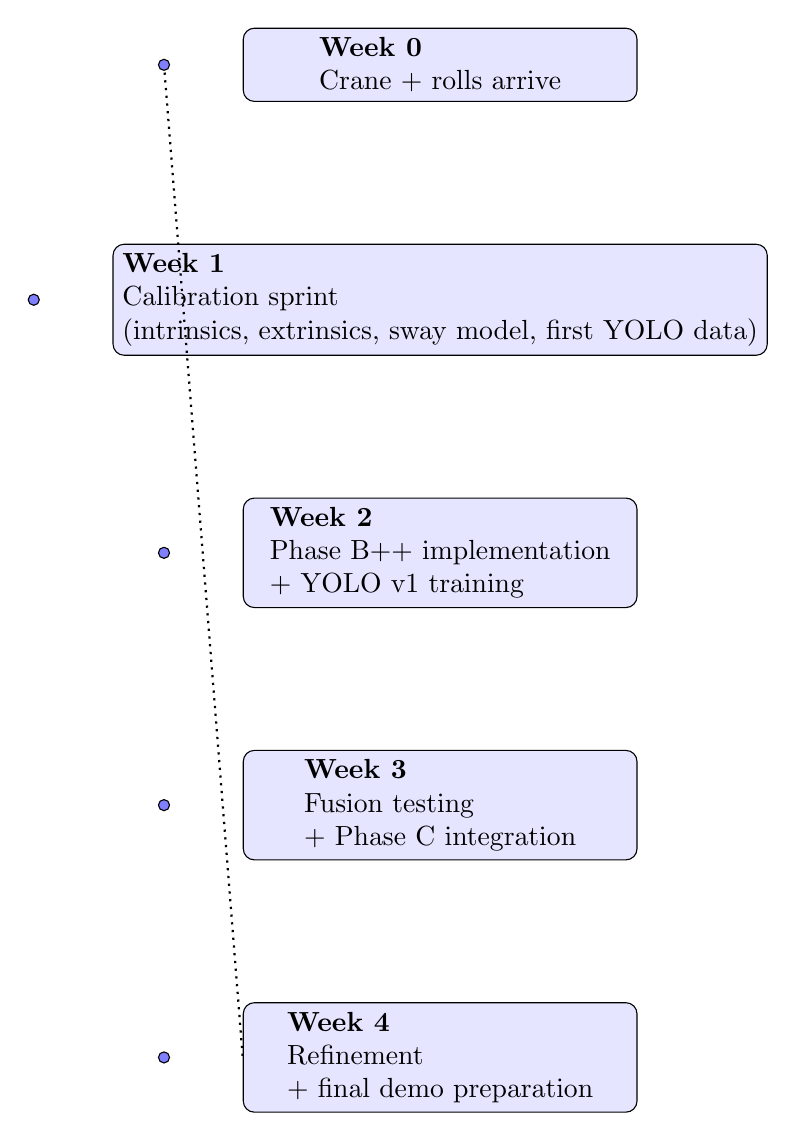
\begin{tikzpicture}[>=Stealth, node distance=1.8cm]
        \tikzstyle{weeknode}=[rectangle, rounded corners, draw=black, fill=blue!10, minimum width=5cm, align=left]
        \node[weeknode] (w0) {\textbf{Week 0}\\Crane + rolls arrive};
        \node[weeknode, below=of w0] (w1) {\textbf{Week 1}\\Calibration sprint\\(intrinsics, extrinsics, sway model, first YOLO data)};
        \node[weeknode, below=of w1] (w2) {\textbf{Week 2}\\Phase B++ implementation\\+ YOLO v1 training};
        \node[weeknode, below=of w2] (w3) {\textbf{Week 3}\\Fusion testing\\+ Phase C integration};
        \node[weeknode, below=of w3] (w4) {\textbf{Week 4}\\Refinement\\+ final demo preparation};
        \draw[thick, dotted] (w0.west) ++(-1,0) -- (w4.west) ++(-1,0);
        \foreach \x in {w0,w1,w2,w3,w4} {
            \draw[fill=blue!50] (\x.west) ++(-1,0) circle (2pt);
        }
    \end{tikzpicture}
    \caption{Vertical timeline for the sway-camera program.}
    \label{fig:timeline}
\end{figure}

\begin{table}[h]
    \centering
    \begin{tabular}{|c|p{0.7\linewidth}|}
        \hline
        \textbf{Week} & \textbf{Main Tasks} \\\hline
        0 & Receive crane hardware and paper rolls; validate mechanical envelope. \\\hline
        1 & Calibration sprint: capture chessboard images, solve intrinsics/extrinsics, log sway motion, fit sway axis, collect first YOLO dataset. \\\hline
        2 & Implement Phase~B++ fusion and train YOLO v1 on synthetic + captured data. \\\hline
        3 & Execute fusion testing with fixed + sway cameras and integrate the Phase~C detection stack. \\\hline
        4 & Refine tuning, address regressions, and prepare the final demo scenario. \\\hline
    \end{tabular}
    \caption{Weekly deliverables for Weeks 0--4.}
    \label{tab:timeline}
\end{table}

\section{Current Work (Simulation Phase)}
We presently operate in a controlled lab setup to validate the sway-camera pipeline:
\begin{itemize}
    \item \textbf{Proxy world frame:} AprilTag family tag36h11, ID~3, size \SI{100}{\milli\meter}, acts as the origin of \{W\}. All captured positions are expressed relative to this tag.
    \item \textbf{Motion logging:} We run \texttt{motion\_logger.py} while manually moving the camera along the intended sway path, keeping Tag~3 visible. The script records per-frame world poses and their relative deltas.
    \item \textbf{Axis fitting:} \texttt{fit\_sway\_axis.py} performs PCA on the absolute positions to obtain the reference point $p_0$ and the unit direction vector $\mathbf{d}_{\text{sway}}$.
    \item \textbf{Extrinsics synthesis:} For any virtual sway coordinate $s$, \texttt{make\_extrinsics\_sway.py} evaluates $p_C(s) = p_0 + s\,\mathbf{d}_{\text{sway}} + p_{\text{offset}}$ and combines it with user-specified yaw/pitch/roll to produce a Phase~B-compatible $T_{WC}$ file.
    \item \textbf{Phase B v2 validation:} The generated extrinsics are fed into \texttt{phase\_b/v2/phase\_b\_tags\_v2.py} together with the shared intrinsics and rig description. We focus on ensuring the roll angle in the world frame remains stable across sway positions.
\end{itemize}
This simulated workflow verifies that world-frame estimates remain coherent before real crane hardware or encoder feedback becomes available.

\end{document}
